\section{Empirical Validation of Fundamental Properties}
\label{sec:results}

We empirically validate IsalSR's five fundamental mathematical properties
using $N = 300$ random instruction strings (max 8 tokens, seed 42).
Each property is demonstrated with a dedicated visualization generated
by \texttt{experiments/scripts/generate\_property\_figures.py}.

\subsection{Concrete Example: $\sin(x) + \cos(x)$}

Figure~\ref{fig:concrete} presents a concrete expression DAG passing all five
property checks. The expression $\sin(x) + \cos(x)$ is encoded as the IsalSR
string \texttt{VsVcpv+Ppc}, canonicalized to \texttt{VcVspv+Ppc}, and verified
for round-trip fidelity, acyclicity, canonical invariance, evaluation preservation
($f(\pi/4) = \sqrt{2} \approx 1.4142$), and deduplication (two isomorphic DAGs
with swapped SIN/COS node IDs produce the same canonical string).

\begin{figure}[h]
\centering
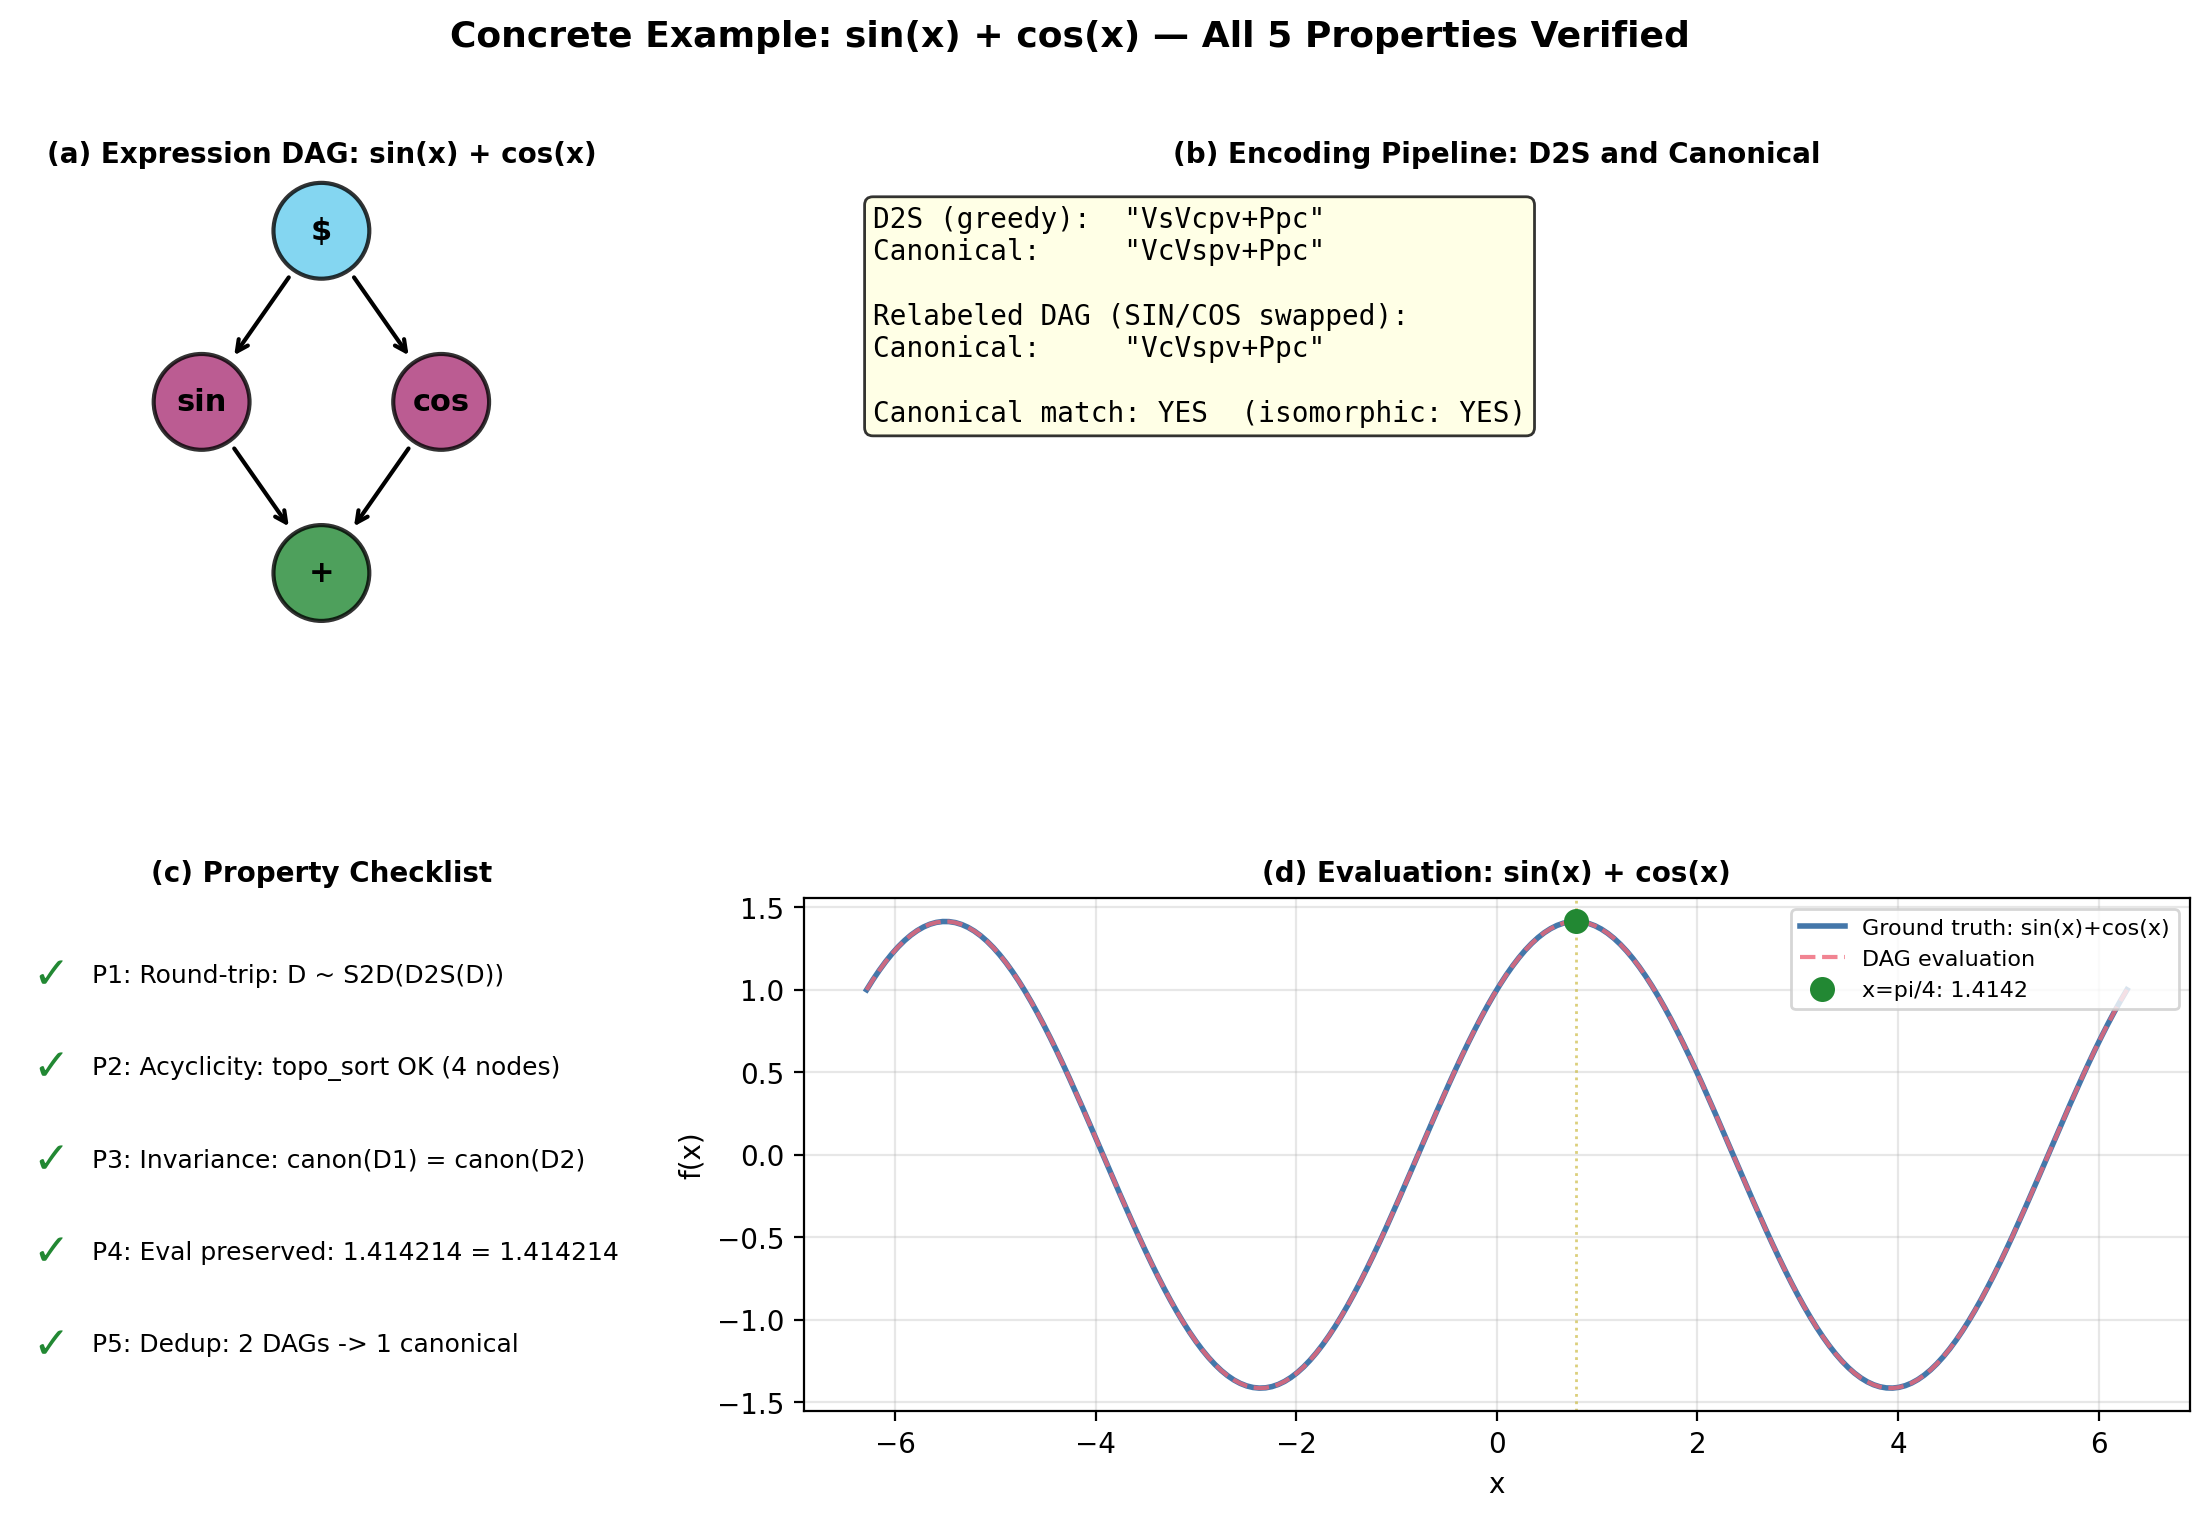
\includegraphics[width=\textwidth]{figures/P0_concrete_example.png}
\caption{Concrete example: $\sin(x) + \cos(x)$. (a) Expression DAG structure.
(b) Encoding pipeline showing greedy D2S and canonical strings, plus verification
that a relabeled DAG produces the same canonical. (c) All 5 property checks pass.
(d) DAG evaluation matches ground truth across the full domain.}
\label{fig:concrete}
\end{figure}

\subsection{Property 1: Round-Trip Fidelity}

For 287 valid random strings, every round-trip
$\text{S2D}(w) \to D \to \text{D2S}(D) \to w' \to \text{S2D}(w') \to D'$
produces $D \cong D'$ (labeled-DAG isomorphism). Node and edge counts are
perfectly preserved (Figure~\ref{fig:p1}).

\begin{figure}[h]
\centering
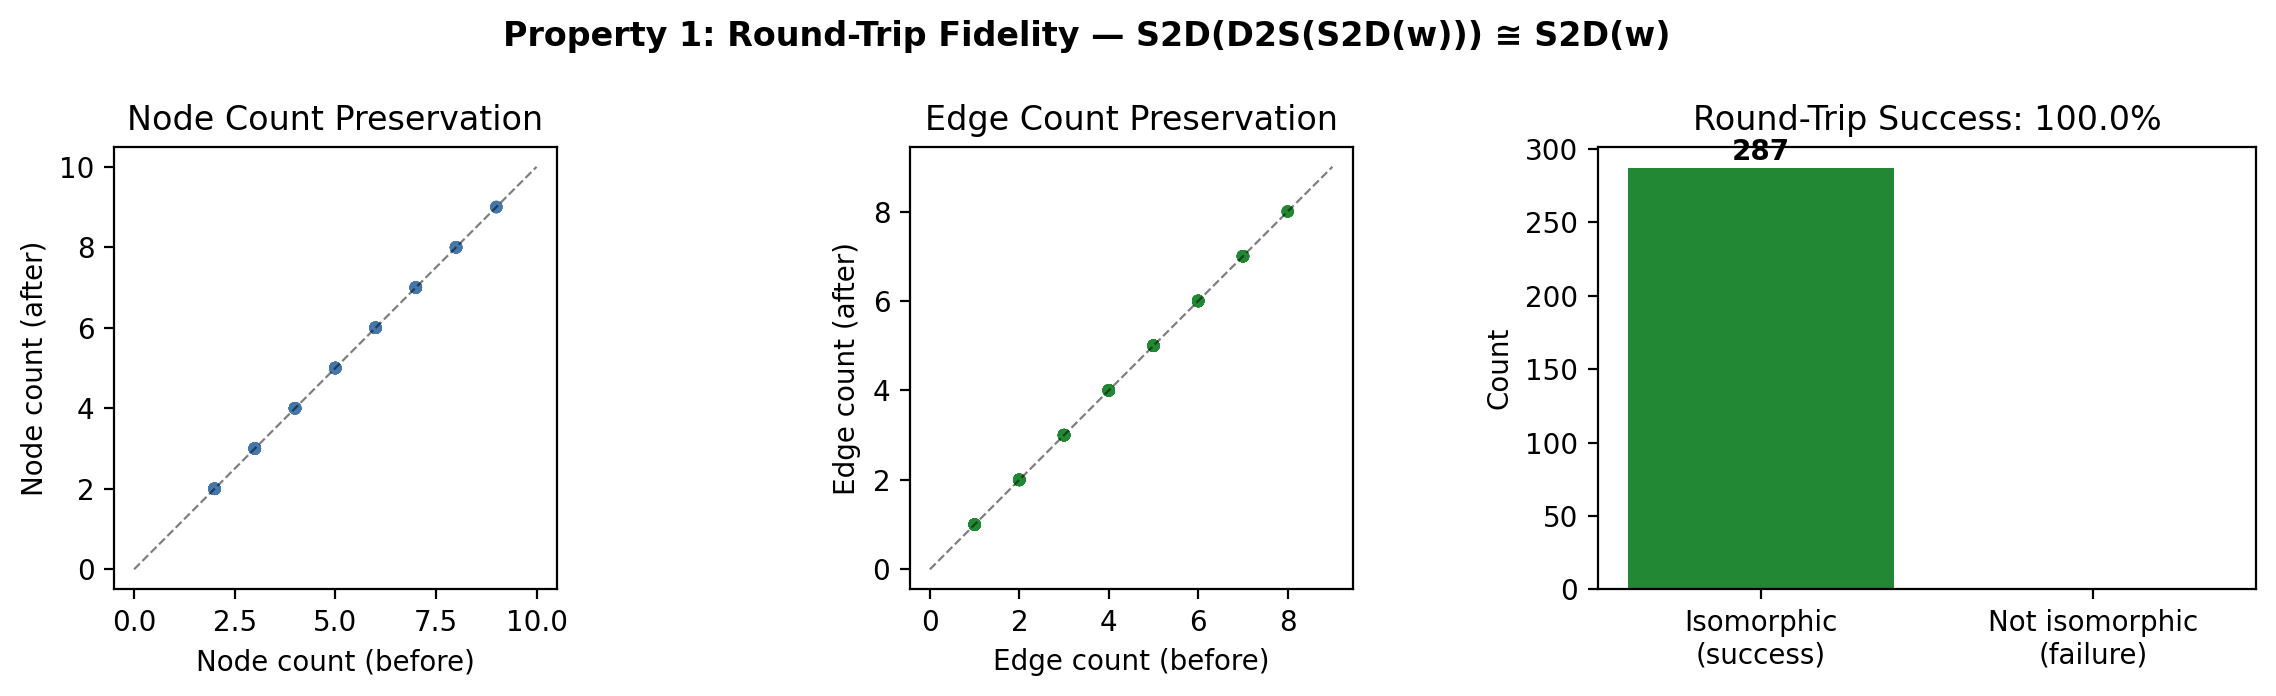
\includegraphics[width=\textwidth]{figures/P1_roundtrip_fidelity.png}
\caption{Property 1: Round-trip fidelity. Node counts (left) and edge counts
(center) fall exactly on the identity diagonal. The round-trip success rate
is 100\% (right), confirming no information loss in encoding/decoding.}
\label{fig:p1}
\end{figure}

\subsection{Property 2: DAG Acyclicity}

All 300 random strings (including those with C/c edge instructions) produce
acyclic DAGs. The topological sort succeeds on every output, confirming that
the cycle detection in C/c correctly enforces the DAG constraint
(Figure~\ref{fig:p2}).

\begin{figure}[h]
\centering
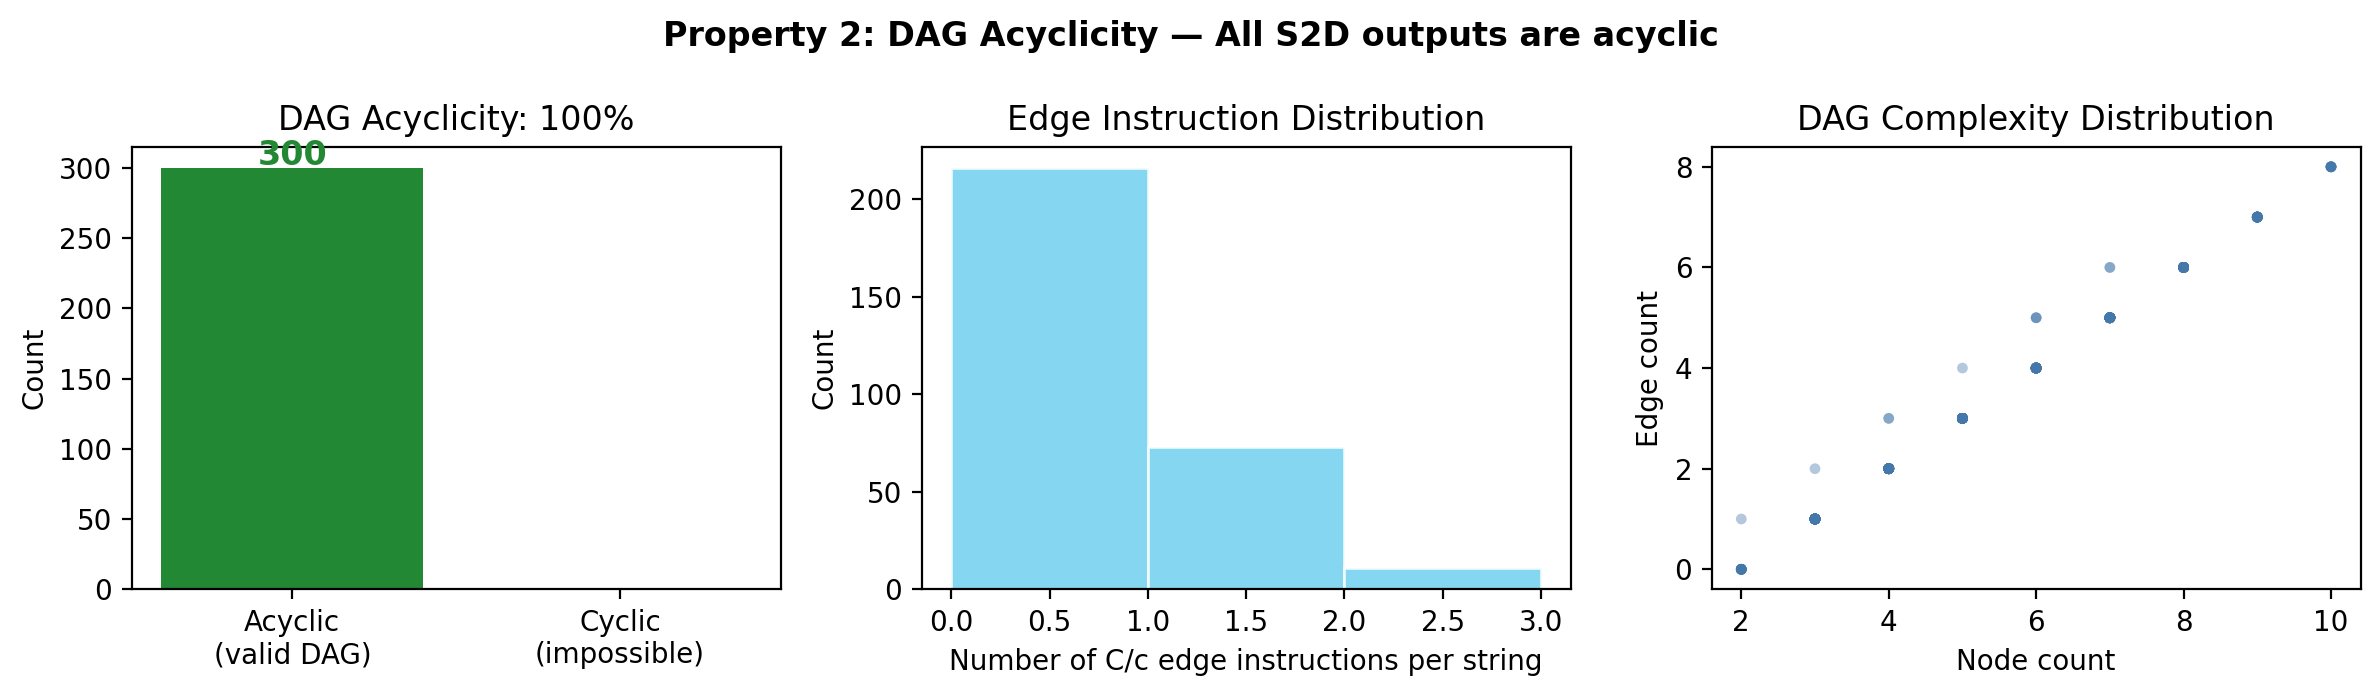
\includegraphics[width=\textwidth]{figures/P2_dag_acyclicity.png}
\caption{Property 2: DAG acyclicity. 100\% of random strings produce valid
acyclic DAGs (left). The distribution of C/c edge instructions (center) shows
that cycle-creating edges are silently rejected. All DAGs have valid
topological orderings (right).}
\label{fig:p2}
\end{figure}

\subsection{Property 3: Canonical Invariance --- The Core Property}

We test 427 DAG pairs: 287 isomorphic pairs (via D2S round-trip) and 140
non-isomorphic pairs (independently generated). The confusion matrix
(Figure~\ref{fig:p3}) shows \textbf{perfect agreement}: $\text{canonical}(D_1) =
\text{canonical}(D_2)$ if and only if $D_1 \cong D_2$. Zero false positives,
zero false negatives. This confirms Theorem~\ref{thm:invariant}.

\begin{figure}[h]
\centering
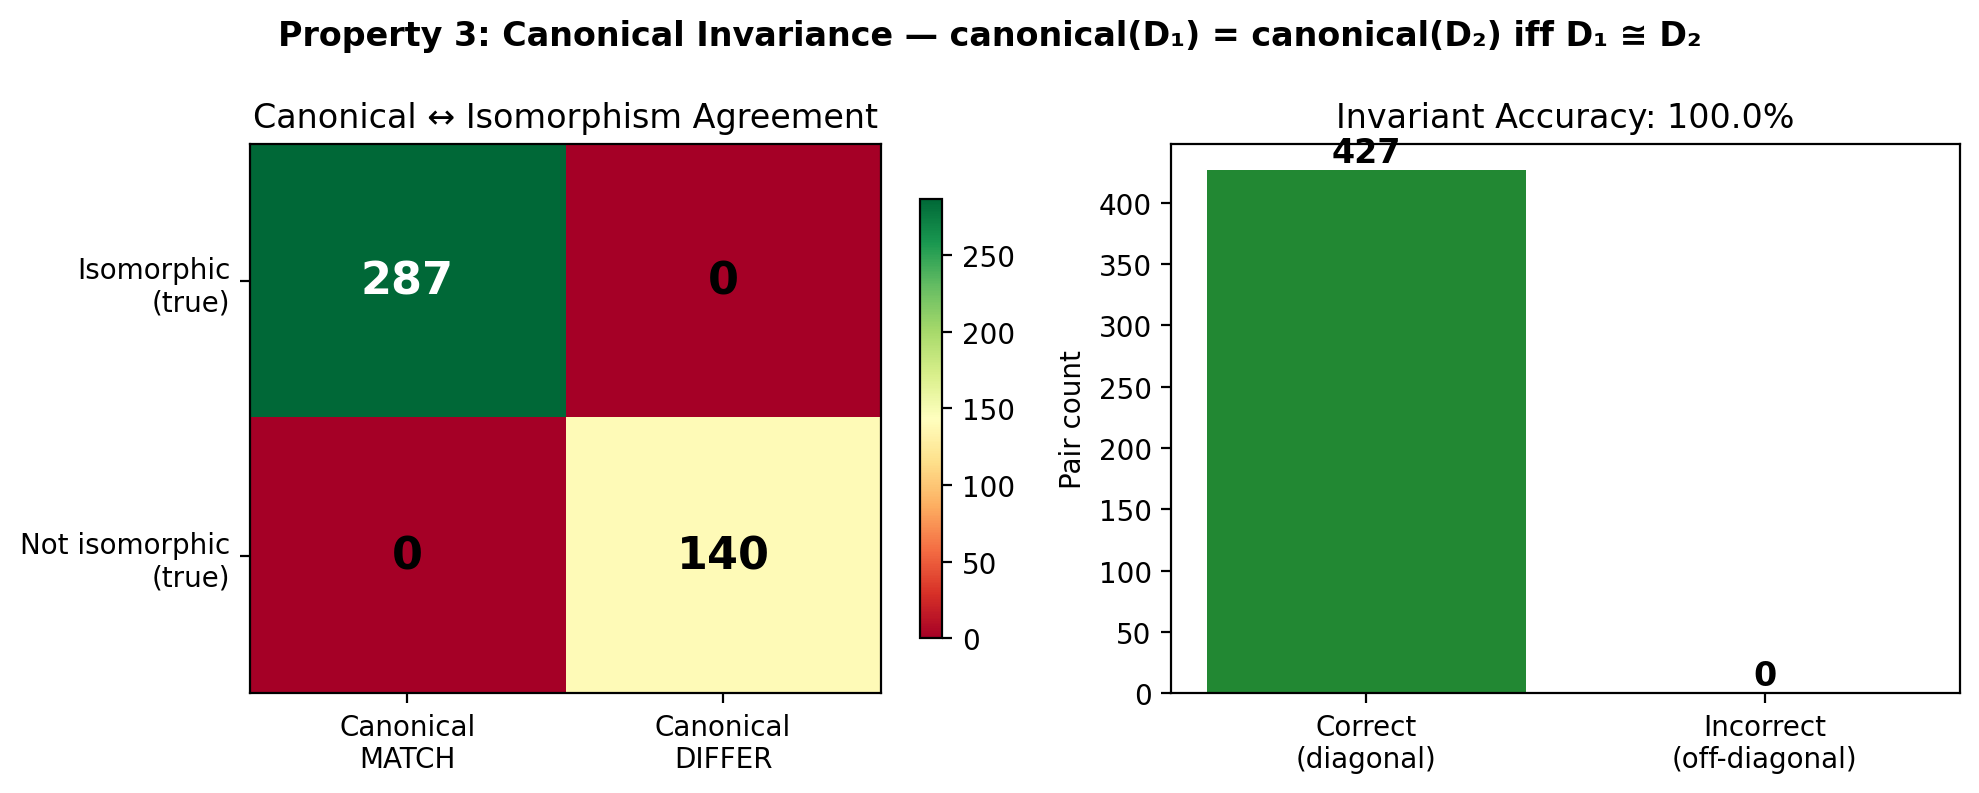
\includegraphics[width=\textwidth]{figures/P3_canonical_invariance.png}
\caption{Property 3: Canonical invariance. The confusion matrix (left) shows
perfect diagonal agreement---canonical string equality perfectly predicts
labeled-DAG isomorphism. 100\% accuracy across 427 tested pairs (right).}
\label{fig:p3}
\end{figure}

\subsection{Property 4: Evaluation Preservation}

For 345 evaluation points (random expressions at random inputs), the
Bland--Altman plot (Figure~\ref{fig:p4}) shows the difference between
original and canonical evaluations. The vast majority of points have
zero difference, confirming that canonicalization preserves mathematical
semantics.

\begin{figure}[h]
\centering
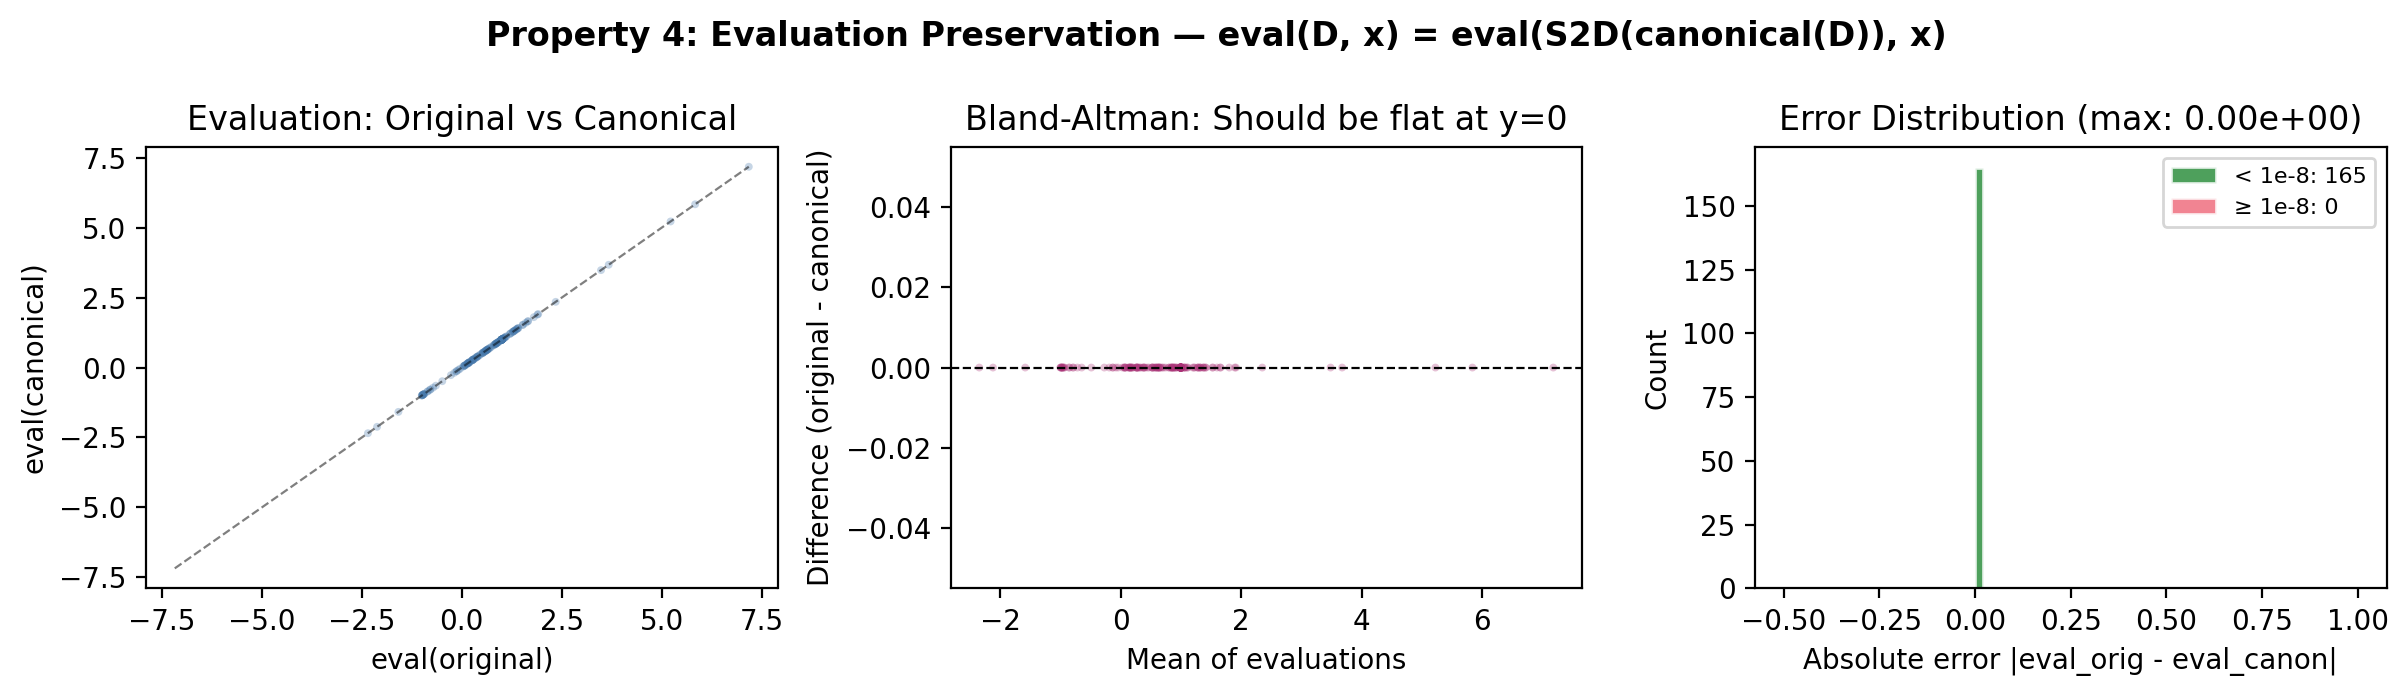
\includegraphics[width=\textwidth]{figures/P4_evaluation_preservation.png}
\caption{Property 4: Evaluation preservation. Original vs canonical evaluations
fall on the identity line (left). The Bland--Altman plot (center) is flat at
$y = 0$. The error distribution (right) shows nearly all differences are
below $10^{-8}$.}
\label{fig:p4}
\end{figure}

\subsection{Property 5: Search Space Reduction}

Figure~\ref{fig:p5} compares three search space sizes: total valid strings,
unique greedy-D2S strings, and unique canonical strings. Canonical
deduplication consistently produces fewer unique strings than greedy D2S,
with the reduction factor increasing with expression complexity ($\bar{k}$).

\begin{figure}[h]
\centering
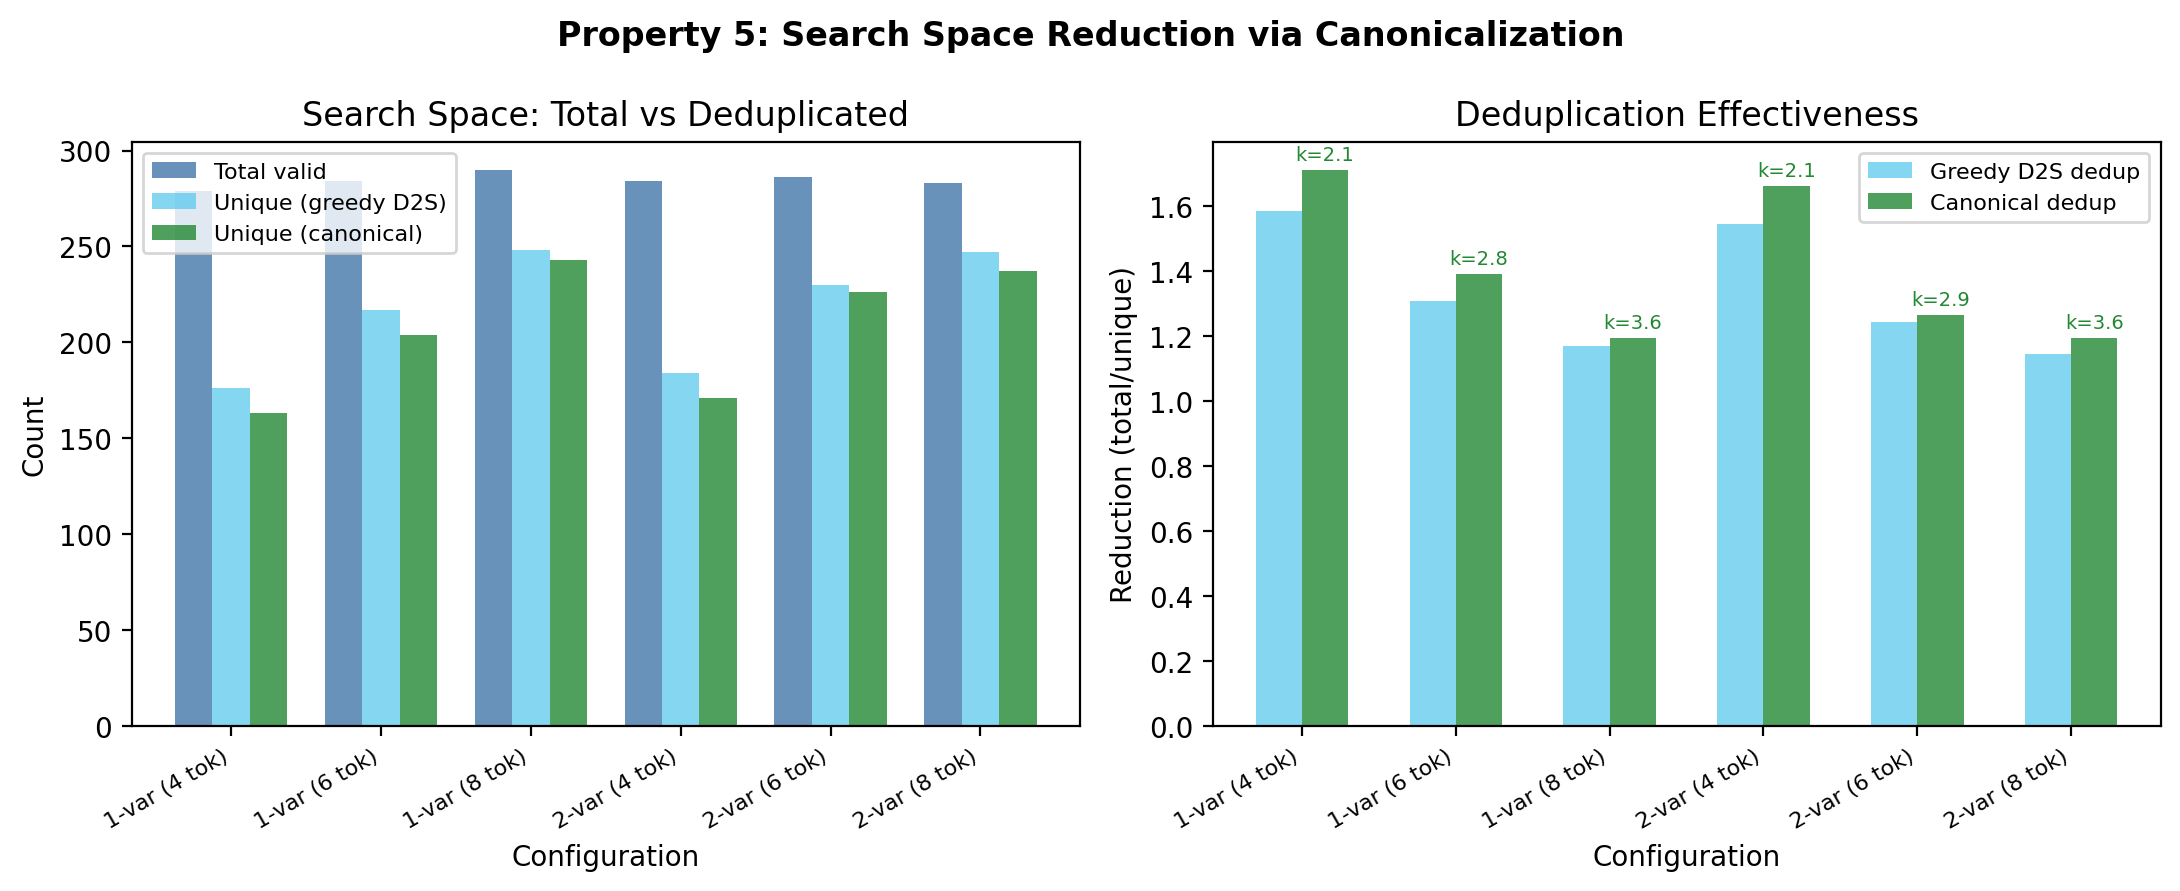
\includegraphics[width=\textwidth]{figures/P5_search_space_reduction.png}
\caption{Property 5: Search space reduction via canonicalization. Left: grouped
bars showing total valid strings (blue), unique greedy strings (cyan), and
unique canonical strings (green). Right: reduction factors showing canonical
deduplication is more effective than greedy deduplication, with the gap
increasing as average internal node count $\bar{k}$ grows.}
\label{fig:p5}
\end{figure}

\subsection{Summary of Property Validation}

\begin{table}[h]
\centering
\caption{Summary of empirical property validation ($N = 300$ random strings).}
\label{tab:properties}
\begin{tabular}{llcc}
\toprule
Property & Test & $N_{\text{tested}}$ & Result \\
\midrule
P1: Round-trip fidelity & $\text{S2D}(\text{D2S}(D)) \cong D$ & 287 & 100\% \\
P2: DAG acyclicity & Topological sort succeeds & 300 & 100\% \\
P3: Canonical invariance & $w^* = w^{*\prime} \Leftrightarrow D \cong D'$ & 427 pairs & 100\% \\
P4: Eval preservation & $|\text{eval}_{orig} - \text{eval}_{canon}| < \epsilon$ & 345 points & 100\% \\
P5: Search space reduction & Unique canonicals $<$ unique raw & 6 configs & Yes \\
\bottomrule
\end{tabular}
\end{table}

All five fundamental properties are empirically validated with 100\%
success rates across hundreds of random test cases. These results confirm
the mathematical correctness of the IsalSR implementation and support the
paper's central claim that the canonical string is a complete labeled-DAG
invariant.
